% author Dinupa Nawarathne
% email dinupa3@gmail.com
% date 09-29-2022


\documentclass[10pt, xcolor={dvipsnames}, aspectratio = 169]{beamer}

%
% use packages
%
\usepackage{graphicx}
\usepackage{amsmath}
\usepackage{hyperref}
\usepackage[absolute,overlay]{textpos}
\usepackage{mathrsfs}
\usepackage{tikz}
\usetikzlibrary{shapes.geometric, arrows}
\usepackage[font=tiny]{caption}
\usepackage{mathrsfs}
\usepackage[backend=bibtex, style=science]{biblatex}
\usepackage{standalone}
\usepackage[most]{tcolorbox}

%
% bib file
%
%\bibliographystyle{plain}
%\bibliography{refs}
\addbibresource{refs.bib}

%
% customization
%
\mode<presentation>
{
% custom colors
\definecolor{nmsured}{RGB}{137,18,22}
% custom fonts
\usefonttheme{serif}
\setbeamercolor{title}{fg=White,bg=nmsured}
\setbeamercolor{frametitle}{fg=White,bg=nmsured}
\setbeamercolor{section number projected}{bg=nmsured,fg=White}
\setbeamercolor{subsection number projected}{bg=nmsured,fg=White}
\setbeamertemplate{items}{\color{nmsured}$\blacksquare$}
\setbeamertemplate{section in toc}[square]
\setbeamertemplate{subsection in toc}[square]
\setbeamertemplate{footline}[frame number]
\setbeamertemplate{caption}[numbered]
\setbeamerfont{footnote}{size=\tiny}
\setbeamercovered{invisible}
\setbeamercolor{block body}{bg=nmsured, fg=White}
\setbeamercolor{block title}{bg=White, fg=nmsured}
}

%
% use this command for citing
%
\newcommand{\citeme}[1]{{\tiny \footfullcite{#1}}}

%
% JPsi partilce
%
\newcommand{\jpsi}{$J/\psi$ }
\newcommand{\pp}{$p\vec{p}$ }

%
% custom tikz commands
%
\tikzstyle{box1} = [rectangle, rounded corners, minimum width=3cm, minimum height=1.5cm,text centered, text width=3cm, draw=BlueGreen, fill=BlueGreen!40]

\tikzstyle{box2} = [rectangle, rounded corners, minimum width=3cm, minimum height=1.5cm,text centered, text width=3cm, draw=Thistle, fill=Thistle!40]

\tikzstyle{box3} = [rectangle, rounded corners, minimum width=3cm, minimum height=1.5cm,text centered, text width=3cm, draw=YellowGreen, fill=YellowGreen!40]

\tikzstyle{arrow} = [ultra thick, BrickRed,->,>=stealth]

%
% title, author, date
%
\title{Extraction of Transverse Single Spin Asymmetry in \jpsi Production in \pp Interactions at 120 GeV Beam Energy}

\author{Dinupa Nawarathne  \and Dr. Vassili Papavassiliou \and Dr. Stephen Pate \\ Forhad Hossain \and Dr. Abinash Pun}

\institute{New Mexico State University \\
Representing the E-1039/SpinQuest
Collaboration}

\date{APS DNP Meeting
\\ October 29, 2022 }

%
% title graphics
%
\titlegraphic{

\includegraphics[width= 3.0 cm]{imgs/Fermilab_logo.svg.png}

\includegraphics[width=1.0cm]{imgs/nmsu.png}
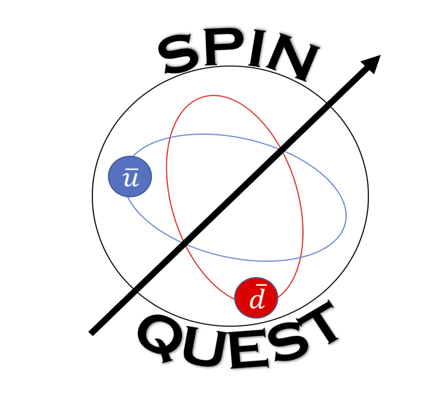
\includegraphics[width=1.5cm]{imgs/spinquest_logo.png}

\includegraphics[width=1.3cm]{imgs/Seal_of_the_United_States_Department_of_Energy.svg.png}
}

%
% begin document
%
\begin{document}

%
% title page
%
\begin{frame}
\maketitle
\end{frame}

%
% table of content
%
\begin{frame}{Overview}
\tableofcontents
\end{frame}

%
% section 2 : TSSA
%
\section{Transverse Single Spin Asymmetry}

\begin{frame}{Transverse Single Spin Asymmetry}

\begin{textblock}{8.0}(0.5, 1.9)

\begin{itemize}

\item In \pp collisions, the transverse single spin asymmetry (TSSA), $A_{N}$, is defined as the amplitude of the
azimuthal angular modulation of the outgoing particle’s scattering cross section with respect to the transverse spin
direction of the polarized proton.

\item The asymmetry can be written as function of azimuthal angle $\phi_{S}$\footnote{\tiny {$\phi_{S}$ is the angle
between $\vec{S}_{\rm target}$ and $\vec{p}_{TJ/\psi}$}.}:
%
\begin{equation*}
    A(\phi_{S}) = \frac{N^{\uparrow}(\phi_{S}) - N^{\downarrow}(\phi_{S})}{N^{\uparrow}(\phi_{S}) + N^{\downarrow}(\phi_{S})} = A_{N}\sin(\phi_{S})
\end{equation*}
%
%
\end{itemize}
\end{textblock}

\begin{textblock}{15.0}(0.5, 11.5)
\begin{itemize}
\item PHENIX results\citeme{PHENIX:2018qvl} shows $A_{N}^{J/\psi}$ \footnote{\tiny{PHENIX convention: $x_{F}$ is measured w.r.t $p$, SpinQuest convention: $x_{F}$ is measured w.r.t. $\vec{p}$.}} as a function of $x_{F}$. In the $p+p$ data a $\sim 2\sigma$ positive $A_{N}$ in the backward higher $x_{F}$ bins. The results for other $x_{F}$ bins are consistent with zero.
\end{itemize}
\end{textblock}

% phenix results

\begin{textblock}{7.0}(8.8, 1.5)

\begin{figure}
    \centering
    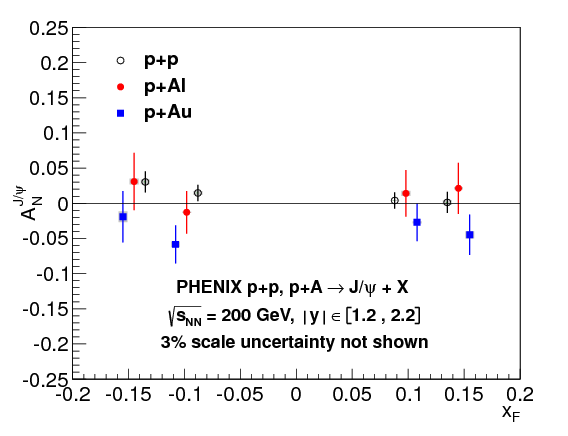
\includegraphics[height = 5.5cm]{imgs/final_xf.png}
    %\caption{PHENIX results for $A^{J/\psi}_{N}$ vs. $x_{F}$. \citeme{PHENIX:2018qvl}}
\end{figure}

\end{textblock}

\end{frame}

%
% section 3: SpinQuest experiment
%

\section{SpinQuest Experiment}

\begin{frame}{SpinQuest Experiment}

\begin{textblock}{9.0}(0.5, 2.0)

\begin{itemize}

\item SpinQuest is a fixed-target Dimuon experiment at Fermilab, using an unpolarized 120 GeV proton beam incident on a
polarized solid ammonia target.

\item SpinQuest measurements will allow us to test models for the internal transverse momentum and angular momentum
structure of the nucleon.

\item In \pp collisions, \jpsi particles are primarily produced by strong interaction with $q\bar{q}$ annihilation and $gg$ fusion.

\item Our goal is to measure $A_{N}$ with an absolute error $\mathcal{O}(10^{-2})$ for a few $p_{T}$ and/or $x_{F}$ bins.

\end{itemize}

\end{textblock}


\begin{textblock}{7.0}(10.0, 2.0)

\begin{figure}
    \centering
    % \includegraphics[width = 0.8\linewidth]{e906_det_3d_run3.pdf}
    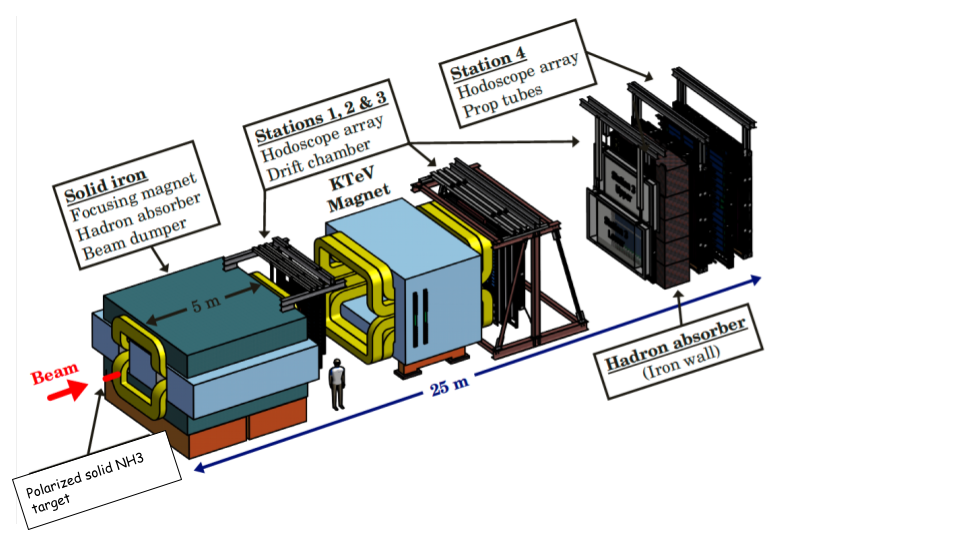
\includegraphics[width = 7.0 cm]{imgs/spectrometer.png}
    \caption{SpinQuest spectrometer. \citeme{SeaQuest:2019hsx}}
\end{figure}
\end{textblock}

\begin{textblock}{14.0}(0.5, 11.0)
\begin{itemize}
    \item In this presentation, we demonstrate the analysis procedure and  extraction of single spin asymmetry ($A_{N}$) with kinematics $0.0 \text{GeV/c}< p_{T} < 2.0 \text{GeV/c}$ and $0.4 < x_{F} < 0.8$.
\end{itemize}
\end{textblock}

\end{frame}

%
%
%
% \begin{frame}{Anticipated Precision of \jpsi TSSA}
%
% \begin{textblock}{7.0}(0.5, 1.2)
% \begin{figure}
%     \centering
%     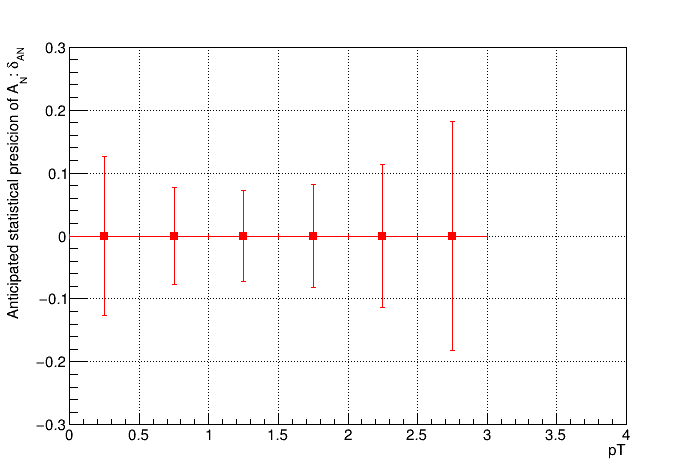
\includegraphics[width = 7.0cm]{imgs/gr_jpsi_tssa_err_pT.png}
%     \caption{Anticipated Precision of $J/\psi$ TSSA for $p_{T}$ bins.}
% \end{figure}
% \end{textblock}
%
% \begin{textblock}{7.0}(8.0, 1.2)
% \begin{figure}
%     \centering
%     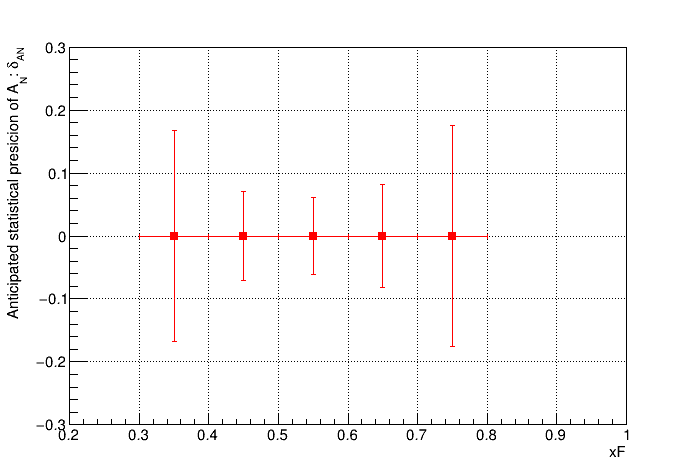
\includegraphics[width = 7.0cm]{imgs/gr_jpsi_tssa_err_xF.png}
%     \caption{Anticipated Precision of \jpsi TSSA for $x_{F}$ bins.}
% \end{figure}
% \end{textblock}
%
% \begin{textblock}{14.0}(0.5, 12.5)
% \begin{itemize}
%     \item For one week of dedicated data taking, a precision of $\sim$ 0.1 is expected. \citeme{kenichi:2021jul}
% \end{itemize}
% \end{textblock}
%
% \begin{textblock}{5.0}(4.0, 2.0)
% {\tiny Monte-Carlo data}
% \end{textblock}
%
% \begin{textblock}{5.0}(12.0, 2.0)
% {\tiny Monte-Carlo data}
% \end{textblock}
%
% \end{frame}

%
%
%
% \begin{frame}{SpinQuest Spectrometer}

% %% spinquest spectrometer
% \begin{textblock}{14.0}(1.0, 1.0)

% \begin{figure}
%     % \centering
%     % \includegraphics[width = 0.8\linewidth]{e906_det_3d_run3.pdf}
%     \begin{tikzpicture}
% \node at (0.5, 1.0) {\includegraphics[width = 12.0 cm, height = 6.5 cm]{imgs/e906_det_3d_run3.pdf}};
% \filldraw[black,ultra thick, fill= White](-5.5,-1.0) rectangle (-2.5,-2.2);
% \node at (-4.0,-1.2) {Polarized solid};
% \node at (-4.0,-1.6) {ammonia target};
% \end{tikzpicture}
%     \caption{SpinQuest spectrometer. \citeme{SeaQuest:2019hsx}}
% \end{figure}
% \end{textblock}

% \end{frame}

%
% Section 4 : Analyis procedure
%
\section{Analysis Procedure}

\subsection{Data Generation}

\begin{frame}[fragile]{Data Generation}

\begin{textblock}{14.0}(0.5, 2.0)

\begin{itemize}

\item Simulated data were generated with kinematics:

\begin{itemize}
\item \jpsi events were considered as signal events.

\begin{verbatim}
xF = [-0.2, 1.0]
\end{verbatim}
where $x_{F}$ is the the Feynman x.

\item Drell-Yan events were considered as background events.
\begin{verbatim}
xF = [-0.2, 1.0]
mass = [1.0, 6.0]
\end{verbatim}
\end{itemize}

\item Asymmetry was introduced by weighting the data;
\begin{align*}
w_{A_{N}} &= 1 + A_{N} \sin(\phi_{S} + \phi_{\rm phase})\\
w_{\text{Total}} &= w_{\text{Gen.}}(mass, x_{F}) \times w_{A_{N}}
\end{align*}

where $\phi_{S}$ is the angle between $\vec{S}_{\rm target}$ and $\vec{p}_{TJ/\psi}$ and $\phi_{\rm phase} = 0.$ for spin up and $\phi_{\rm phase} = \pi$ for spin down.

\item Asymmetry values are set as $A_{N}^{J/\psi} = 0.2$ for \jpsi events and $A_{N}^{BG} = 0.1$ for Drell-Yan events.\footnote{\tiny{Dilution factor of the NH3 was not considered in this study.}}

\end{itemize}
\end{textblock}

% \begin{textblock}{5.0}(11.0, 2.0)
% \begin{figure}
%     \centering
%     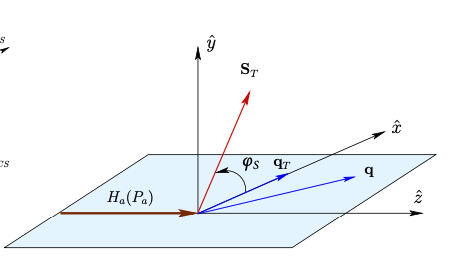
\includegraphics[width = 5.0 cm]{imgs/phi_angle.png}
%     \caption{$\phi_{S}$ definition in the target rest frame.\citeme{Longo:2017snu}}
% \end{figure}
% \end{textblock}

\end{frame}

\begin{frame}{Analysis Procedure}

\begin{textblock}{14.0}(0.5, 1.5)

\begin{figure}
    \centering
    %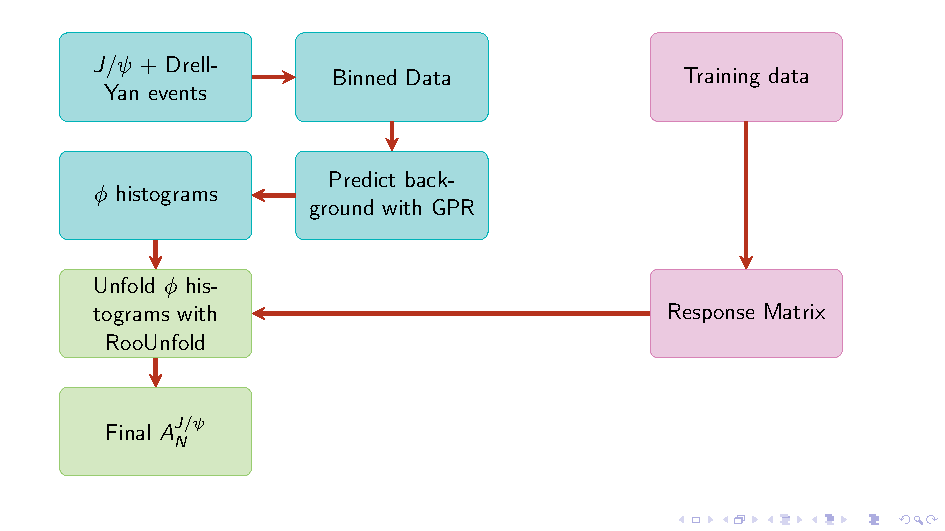
\includegraphics[width = 0.9\linewidth]{flowchart.pdf}
    \includestandalone[width=0.95\linewidth]{flowchart}
    %\caption{Analysis procedure.}
\end{figure}

\end{textblock}

\end{frame}


%
% Subsection : GPR
%

\subsection{Gaussian Process Regression (GPR)}

\begin{frame}[fragile]{Gaussian Process Regression (GPR)}

\begin{textblock}{14.0}(0.5, 2.0)
\begin{itemize}

\item The Gaussian process model is a probabilistic supervised machine learning technique used in classification and regression tasks. A Gaussian process regression (GPR) model can make predictions incorporating prior knowledge (kernels) and provide uncertainties of the predictions.\citeme{10.7551/mitpress/3206.001.0001}

\item In this analysis, the Radial-Basis Function (RBF) kernel was used as the kernel function in GPR class in \verb|sklearn| library.

\begin{equation*}
k(x_{i}, x_{j}) = \exp\left[-\frac{d^{2}(x_{i}, x_{j})}{2l^{2}}\right]
\end{equation*}

where $l$ is the length scale of the kernel and $d(\cdot,\cdot)$ is the Euclidean distance.\citeme{pedregosa2011scikit}

\item We fit this kernel in side-band regions on either side of the \jpsi invariant mass peak. Then we used the trained kernel  to predict the background in the \jpsi peak region.

\item \textcolor{blue}{\textbf{Our first goal is to extract the background under the \jpsi peak using the GPR method with good statistical precision}}.

\end{itemize}
\end{textblock}

\end{frame}

%
%
%

\begin{frame}{Sanity Check}

\begin{textblock}{7.0}(0.5, 1.5)
\begin{figure}
    \centering
    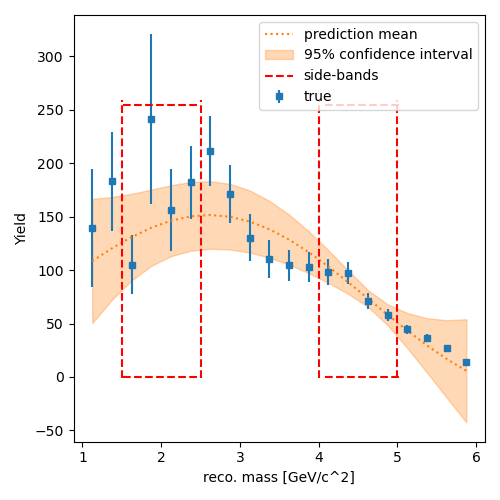
\includegraphics[width=7.0cm]{imgs/mass_pt.png}
    \caption{GPR prediction for background. The side-bands are given in the red dashed lines.}
\end{figure}
\end{textblock}

\begin{textblock}{7.0}(8.0, 3.0)
\begin{itemize}

  \item We used the Drell-Yan mass distribution in different $p_{T}$ and $x_{F}$ bins to check the GPR prediction.background

  \item \textcolor{blue}{\textbf{As shown in figure 9, the prediction from GPR method agrees with the Drell-Yan events with 95\% confidence interval in the \jpsi mass region}}.

\end{itemize}
\end{textblock}

\end{frame}


\begin{frame}{Predicted Background}

\begin{textblock}{7.0}(0.5, 1.2)
\begin{figure}
    \centering
    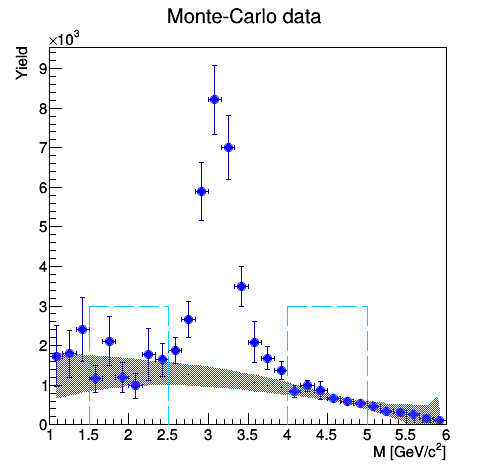
\includegraphics[width = 1.0\linewidth]{imgs/mass_hist000.png}
    \caption{Mass histogram for 1st $p_{T}$ bin and 1st $\phi$ bin. Predicted background is given in shaded red region. Side-bands are indicated in dashed blue lines.}
\end{figure}
\end{textblock}

\begin{textblock}{7.0}(8.0, 1.2)
\begin{figure}
    \centering
    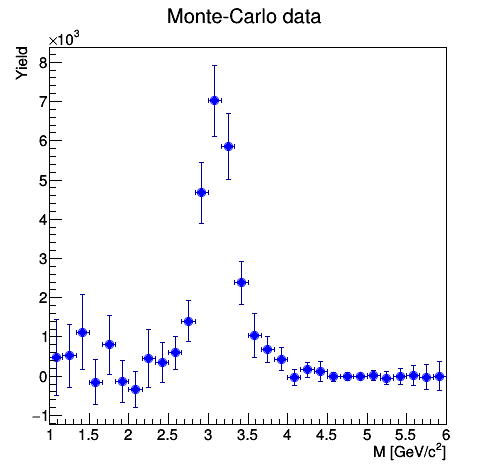
\includegraphics[width = 1.0\linewidth]{imgs/signal_hist000.png}
    \caption{\jpsi signal after subtracting the background.}
\end{figure}
\end{textblock}

\end{frame}

%
% Subsection : ROOUnfold
%

\subsection{RooUnfold}

\begin{frame}[fragile]{Unfolding $\phi$ Distributions}

\begin{textblock}{14.0}(0.5, 2.0)

\begin{itemize}

\item Unfolding in high energy physics represents the correction of measured spectra in data for the finite detector
efficiency, acceptance, and resolution from the detector to particle level.

\item The equation of unfolding \footfullcite{Baron:2021vvl};

\begin{equation*}
\vec{P} = \frac{1}{\epsilon} M^{-1} \eta (\vec{D}-\vec{B})
\end{equation*}

where $\vec{D}$ is the data spectrum, $\vec{B}$ is the background spectrum, $\eta$ acceptance correction, $M^{-1}$ is the migration matrix, $\epsilon$ is the detector efficiency and $\vec{P}$ is the unfolded spectrum.

% \item We used the \verb|RooUnfold| package in the analysis. Some default algorithms are:
%
% \begin{itemize}
%     \item Iterative Bayesian
%     \item Singular value decomposition
%     \item Bin-by-bin (simple correction factors)
% \end{itemize}

\item We trained the response matrix with Drell-Yan events without any asymmetry included. We used the iterative Bayesian method in \verb|ROOUnfold| library to unfold the $\phi$ distributions. \citeme{Wynne:2012jb}
\item \textcolor{blue}{\textbf{Our second goal is to correct the bin-by-bin migration using the iterative Bayesian unfolding}}.

\end{itemize}

\end{textblock}

\end{frame}

% \begin{frame}{RooUnfold}
% \begin{textblock}{14.0}(0.5, 2.5)
% \begin{itemize}
%     \item We trained the response matrix with Drell-Yan events without any asymmetry included.
%     \item We used the iterative Bayesian method to unfold the $\phi$ distributions. \citeme{Wynne:2012jb}
%     \item By using the unfolding method we will correct the bin-by-bin migration.
% \end{itemize}
% \end{textblock}
% \end{frame}

%
%
%
\begin{frame}{Response Matrix for $p_{T}$ Bins}

\begin{textblock}{7.0}(0.5, 2.0)
\begin{figure}
    \centering
    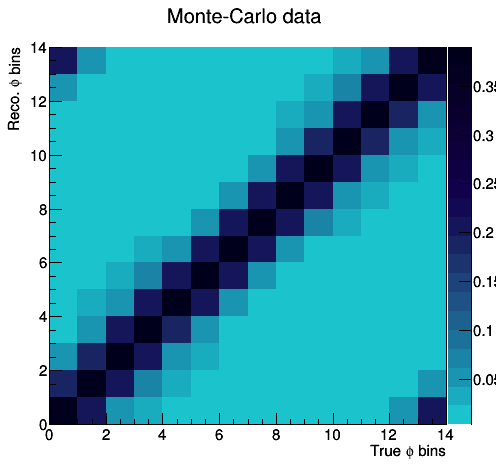
\includegraphics[width = 1.0\linewidth]{imgs/matrix_pt0.png}
    \caption{Reco. $\phi$ vs. true $\phi$.}
\end{figure}
\end{textblock}

\begin{textblock}{7.0}(8.0, 2.0)
\begin{figure}
    \centering
    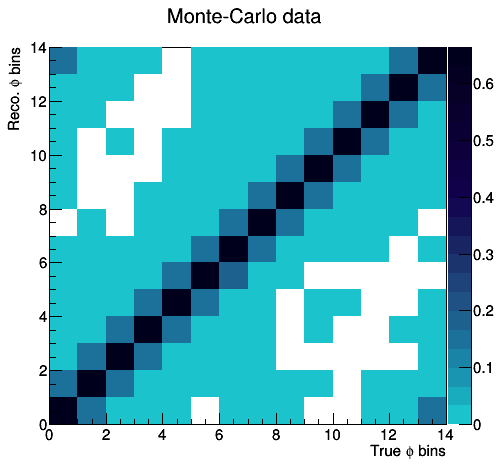
\includegraphics[width = 1.0\linewidth]{imgs/matrix_pt1.png}
    \caption{Reco. $\phi$ vs. true $\phi$.}
\end{figure}
\end{textblock}

\begin{textblock}{3.0}(5.5, 3.0)
$\color{red} 0.0 < p_{T} < 1.0$
\end{textblock}

\begin{textblock}{3.0}(13.0, 3.0)
$\color{red} 1.0 < p_{T} < 2.0$
\end{textblock}

\end{frame}

\begin{frame}{Response Matrix for $x_{F}$ Bins}

\begin{textblock}{7.0}(0.5, 2.0)
\begin{figure}
    \centering
    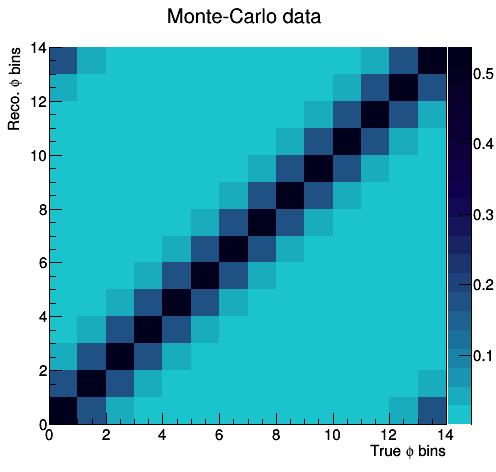
\includegraphics[width = 1.0\linewidth]{imgs/matrix_xf0.png}
    \caption{Reco. $\phi$ vs. true $\phi$.}
\end{figure}
\end{textblock}

\begin{textblock}{7.0}(8.0, 2.0)
\begin{figure}
    \centering
    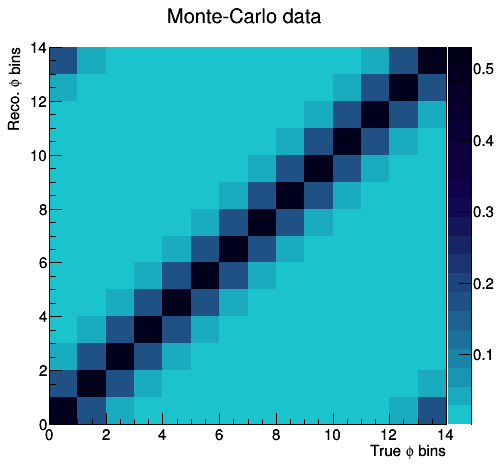
\includegraphics[width = 1.0\linewidth]{imgs/matrix_xf1.png}
    \caption{Reco. $\phi$ vs. true $\phi$.}
\end{figure}
\end{textblock}

\begin{textblock}{3.0}(5.5, 3.0)
$\color{red} 0.4 < x_{F} < 0.6$
\end{textblock}

\begin{textblock}{3.0}(13.0, 3.0)
$\color{red} 0.6 < x_{F} < 0.8$
\end{textblock}

\end{frame}

%
% Section 5 : Results and Discussion
%
\section{Results and Discussion}

%% slide 16

\begin{frame}{Unfolded $A^{J/\psi}_{N}$ in $p_{T}$ Bins}

\begin{textblock}{7.0}(0.5, 2.0)
\begin{figure}
    \centering
    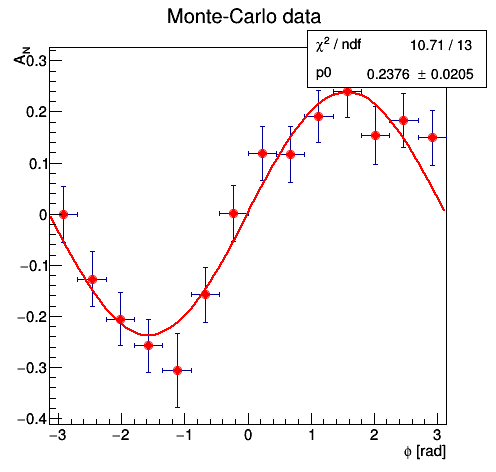
\includegraphics[width = 1.0\linewidth]{imgs/sigal_asym0.png}
    \caption{Unfolded asymmetry.}
\end{figure}
\end{textblock}

\begin{textblock}{7.0}(8.0, 2.0)
\begin{figure}
    \centering
    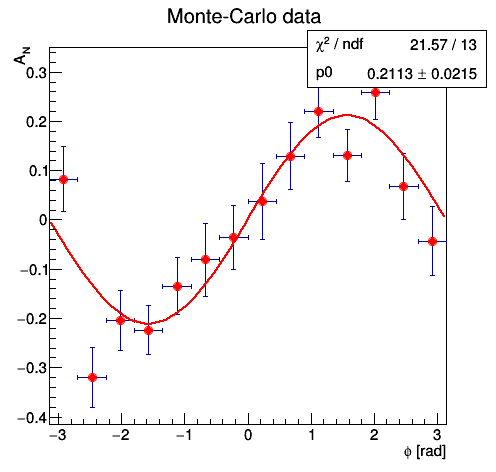
\includegraphics[width = 1.0\linewidth]{imgs/sigal_asym1.png}
    \caption{Unfolded asymmetry.}
\end{figure}
\end{textblock}

\begin{textblock}{3.0}(0.5, 3.0)
$\color{red} 0.0 < p_{T} < 1.0$
\end{textblock}

\begin{textblock}{3.0}(8.0, 3.0)
$\color{red} 1.0 < p_{T} < 2.0$
\end{textblock}

\begin{textblock}{5.0}(4.0, 11.0)
\begin{small}
\textcolor{blue}{\textbf{Generated $A_{N} = 0.2$ \\
Extracted $A_{N} = 0.238 \pm 0.021$}}
\end{small}
\end{textblock}

\begin{textblock}{5.0}(11.0, 11.0)
\begin{small}
\textcolor{blue}{\textbf{Generated $A_{N} = 0.2$ \\
Extracted $A_{N} = 0.211 \pm 0.022$}}
\end{small}
\end{textblock}

\end{frame}

\begin{frame}{Unfolded $A^{J/\psi}_{N}$ in $x_{F}$ Bins}

\begin{textblock}{7.0}(0.5, 2.0)
\begin{figure}
    \centering
    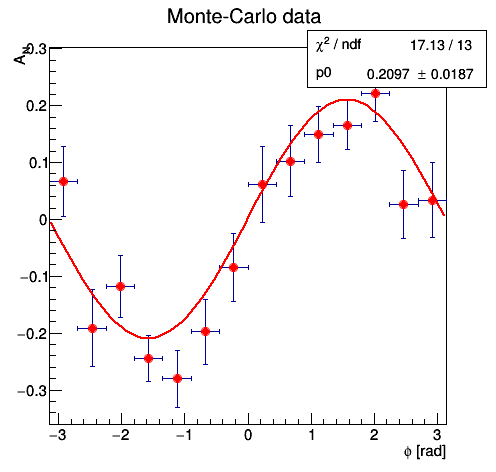
\includegraphics[width = 1.0\linewidth]{imgs/sigal_asym_xf0.png}
    \caption{Unfolded asymmetry.}
\end{figure}
\end{textblock}

\begin{textblock}{7.0}(8.0, 2.0)
\begin{figure}
    \centering
    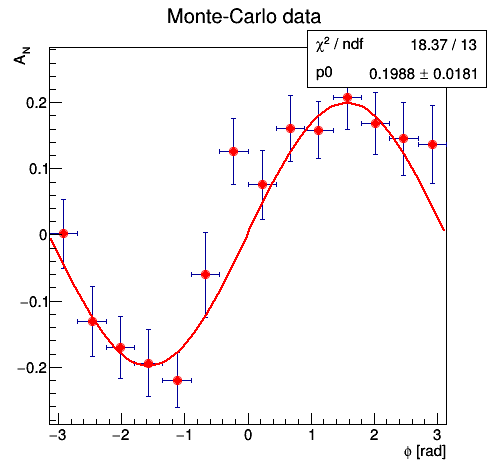
\includegraphics[width = 1.0\linewidth]{imgs/sigal_asym_xf1.png}
    \caption{Unfolded asymmetry.}
\end{figure}
\end{textblock}

\begin{textblock}{3.0}(0.5, 3.0)
$\color{red} 0.4 < x_{F} < 0.6$
\end{textblock}

\begin{textblock}{3.0}(8.0, 3.0)
$\color{red} 0.6 < x_{F} < 0.8$
\end{textblock}

\begin{textblock}{5.0}(4.0, 11.0)
\begin{small}
\textcolor{blue}{\textbf{Generated $A_{N} = 0.2$ \\
Extracted $A_{N} = 0.210 \pm 0.019$}}
\end{small}
\end{textblock}

\begin{textblock}{5.0}(11.0, 11.0)
\begin{small}
\textcolor{blue}{\textbf{Generated $A_{N} = 0.2$ \\
Extracted $A_{N} = 0.199 \pm 0.018$}}
\end{small}
\end{textblock}

\end{frame}

\begin{frame}{Extracted $A_{N}$}

\begin{textblock}{7.0}(0.5, 1.5)
\begin{figure}
    \centering
    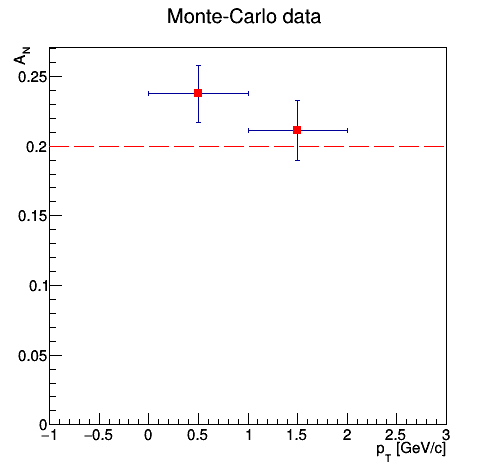
\includegraphics[width = 1.0\linewidth]{imgs/final_asym_pt.png}
    \caption{Extracted asymmetry for $p_{T}$ bins. Generated asymmetry is shown in red dashed line.}
\end{figure}
\end{textblock}

\begin{textblock}{7.0}(8.0, 1.5)
\begin{figure}
    \centering
    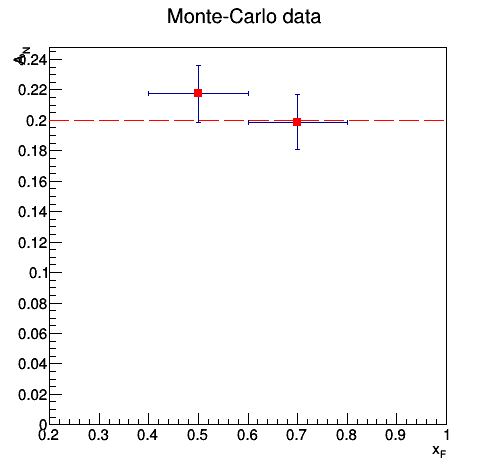
\includegraphics[width = 1.0\linewidth]{imgs/final_asym_xf.png}
    \caption{Extracted asymmetry for $x_{F}$ bins. Generated asymmetry is shown in red dashed line.}
\end{figure}
\end{textblock}

\begin{textblock}{5.0}(11.0, 8.0)
\begin{small}
\textcolor{blue}{\textbf{Generated $A_{N} = \text{0.2}$ \\
Extracted asymmetry reproduces the generated asymmetry within a $\sim \sigma$ confidence interval.}}
\end{small}
\end{textblock}

\end{frame}

%
% Summary
%
\section{Summary}

\begin{frame}{Summary}

\begin{textblock}{15.0}(0.5, 2.0)

\begin{itemize}

\item Gaussian process regression (GPR) is a supervised machine learning method that can be used to predict the background under the \jpsi peak.

\item Using GPR method with the RBF kernel, background of the \jpsi mass can be predicted with 95\% confidence interval.

\item Using iterative Bayesian unfolding we can correct the bin-by-bin migration.

\item Using these techniques (GPR+Unfolding), the extracted asymmetry reproduces the generated asymmetry within a $\sim \sigma$
confidence interval.

\item  SpinQuest does not overlap with PHENIX kinematics.

\begin{itemize}

    \item In PHENIX $|x_{F}| < 0.3$

    \item In SpinQuest $|x_{F}| > 0.4$

\end{itemize}

SpinQuest  will explore a new region of kinematics. Measurement for \jpsi transverse single spin asymmetry can be extracted in a few weeks of data taking with good statistical precision.

\item Acknowledgement:

\begin{itemize}
    \item This work is supported by the US Department of Energy, Office of Science, Medium Energy Nuclear Physics Program.
\end{itemize}

\end{itemize}

\end{textblock}

\end{frame}

%
%
% BACKUP slides
%
%
%

\begin{frame}
\begin{block}
{Backup Slides}
\end{block}
\end{frame}


%
% section 1 : jpsi particle
%
%\section{\jpsi Particle}

\begin{frame}{\jpsi Particle}

\begin{textblock}{10.0}(0.5, 2.0)

\begin{itemize}

\item \jpsi is a vector meson which is a $c\bar{c}$ bound state.

\item Discovered by Burton Richter and Samuel Ting in 1974. Awarded Nobel price for the discovery in 1976.

\item In \pp collisions, \jpsi particles are primarily produced by strong interaction with $q\bar{q}$ annihilation and $gg$ fusion.

\end{itemize}

\end{textblock}

%
% jpsi mass picture
%
\begin{textblock}{5.0}(10.5, 1.5)
\begin{figure}
    \centering
    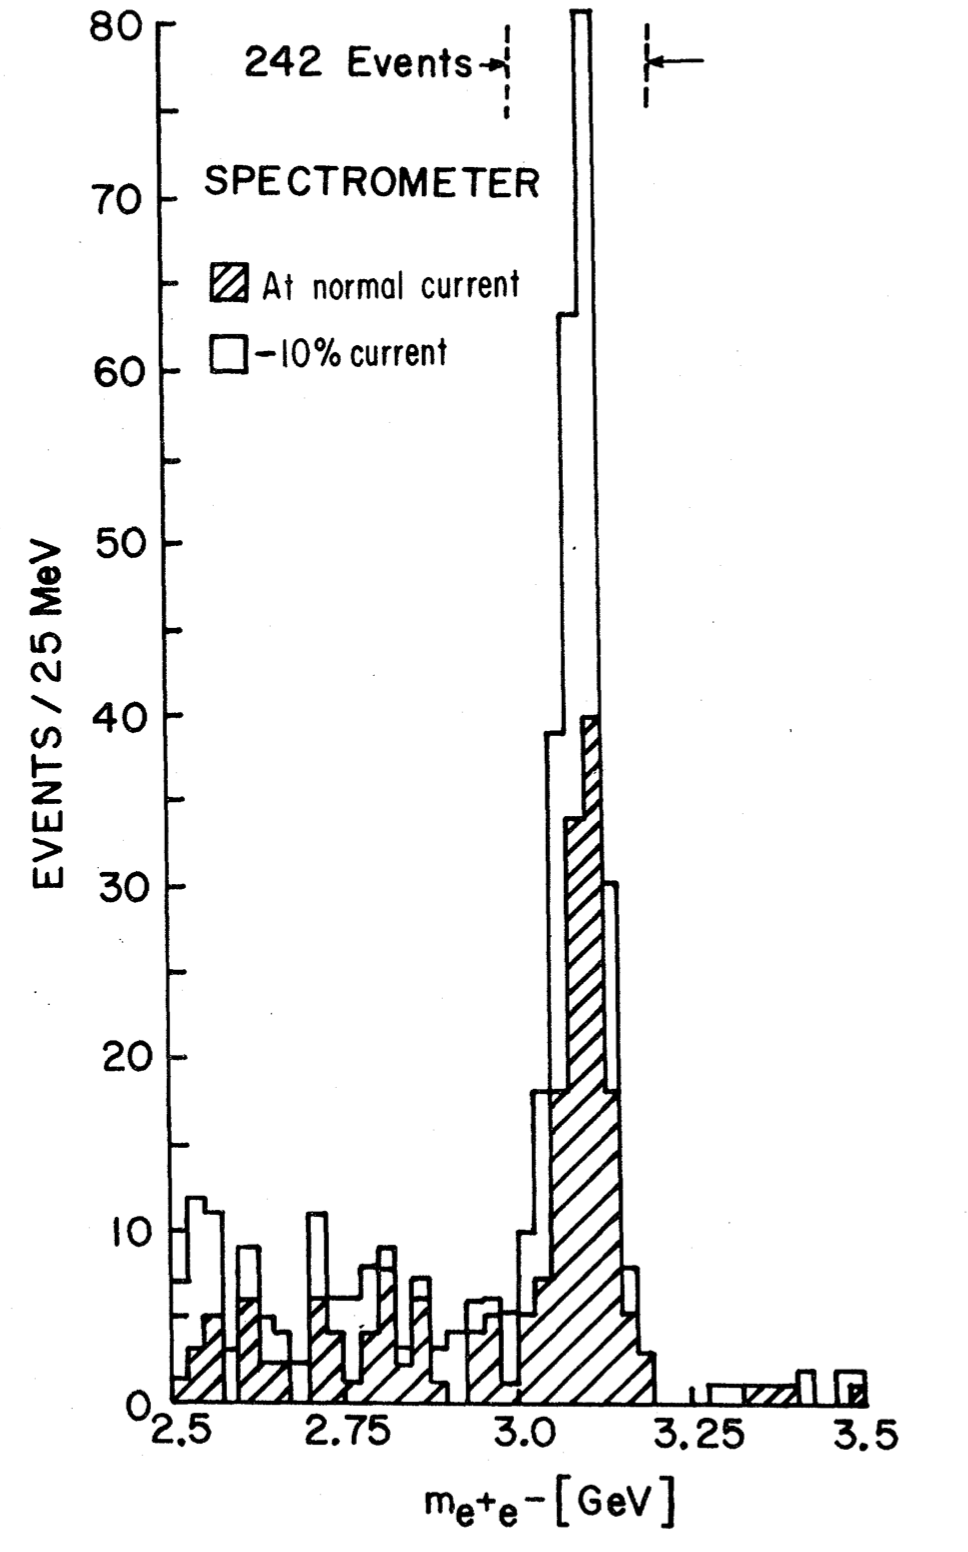
\includegraphics[height = 6.0cm]{imgs/jpsi.png}
    \caption{Mass spectrum showing the existence of \jpsi.\citeme{Aubert:1976oaa}}
\end{figure}
\end{textblock}

%
% properties table
%
\begin{textblock}{8.0}(1.0, 6.5)
\begin{figure}
    \centering
    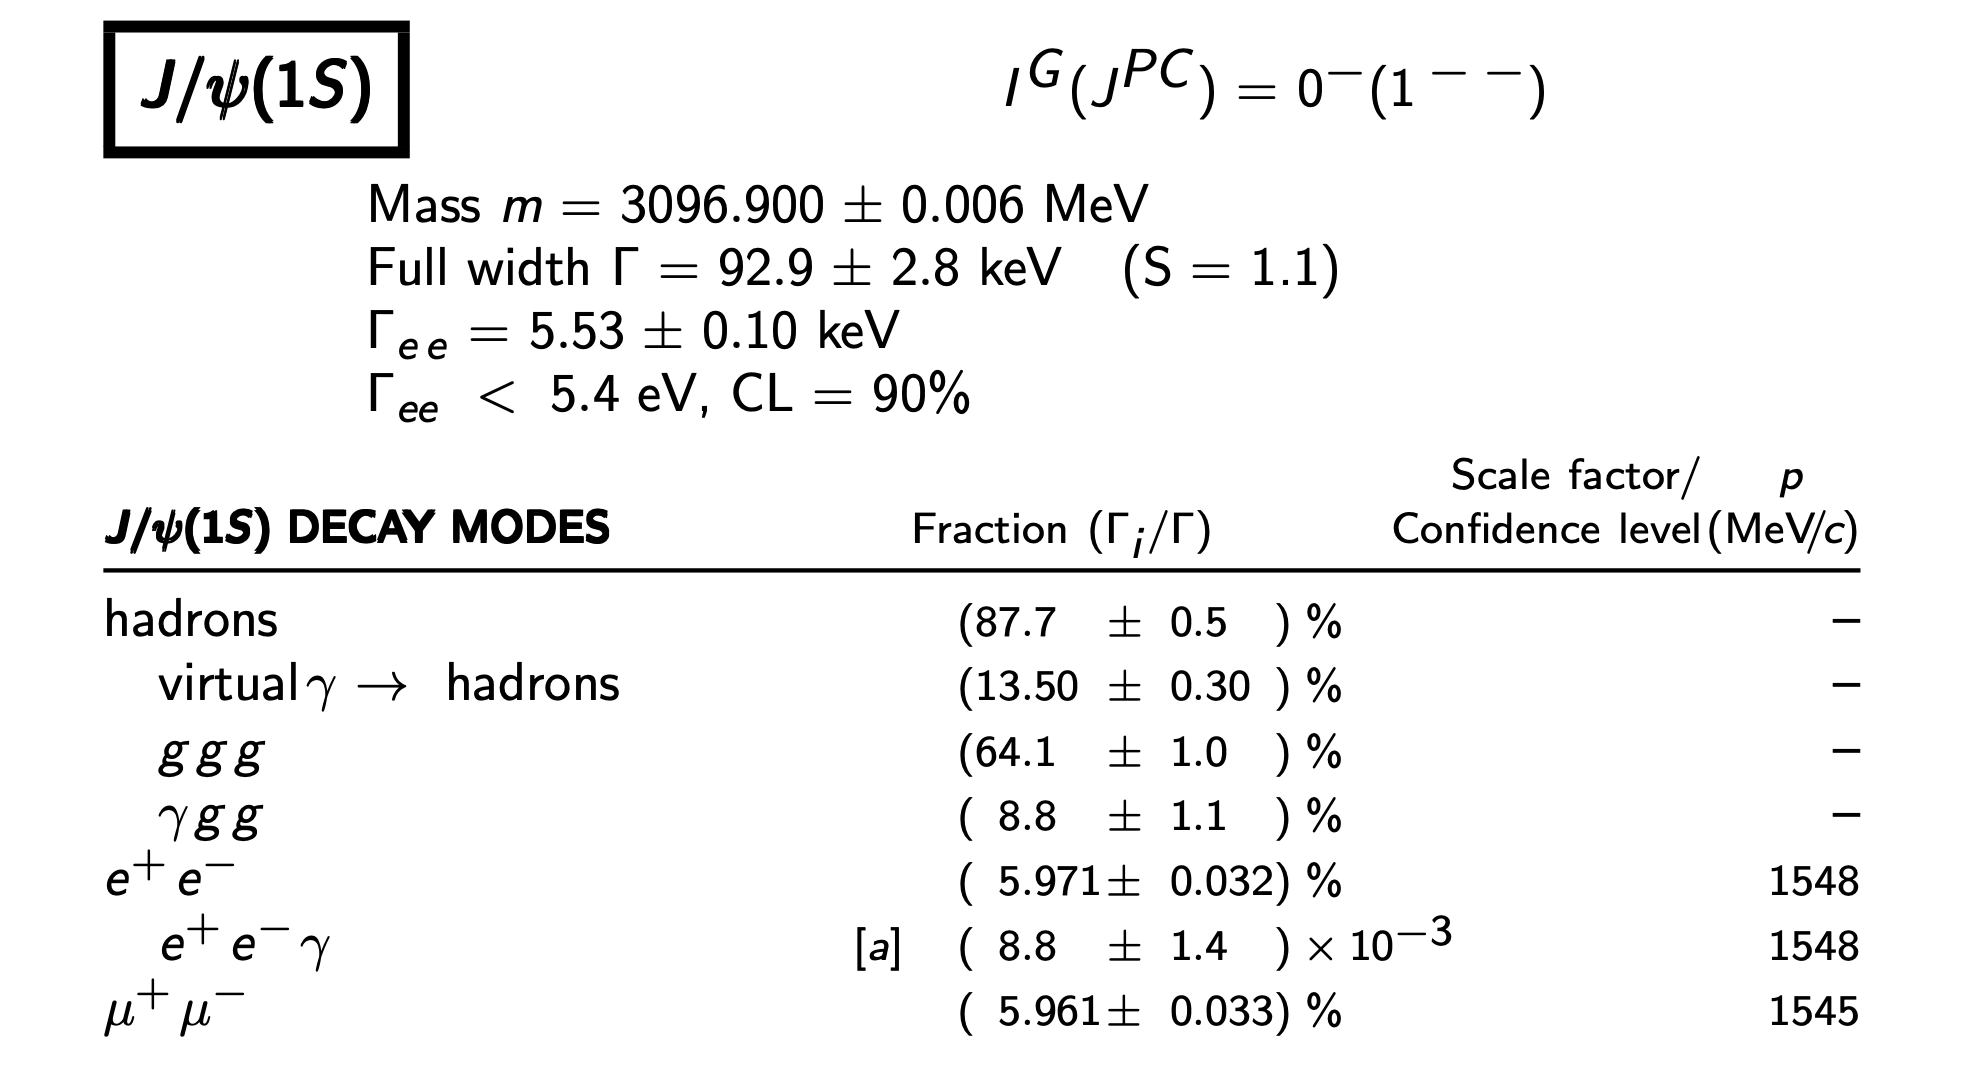
\includegraphics[height = 3.5cm]{imgs/properties.png}
    \caption{\jpsi properties.\citeme{ParticleDataGroup:2020ssz}}
\end{figure}
\end{textblock}
\end{frame}


%
% subsection 1.1 : JPsi production
%

% \subsection{\jpsi Production}

\begin{frame}{\jpsi Production}
\begin{textblock}{14.0}(0.5, 2.0)

Color evaporation model (CEM), Color Singlet model (CSM) and Color Octet model (COM) are three most prominent models
developed to understand the production of \jpsi particle. All three models attempt to factorize the \jpsi production
into a relativistic part describing the production of $c\bar{c}$ $d\sigma_{c\bar{c}[n]}$, and a non-relativistic part
describing the bound state of two quarks $F_{c\bar{c}[n]}(\Lambda)$;

\begin{equation*}
d\sigma (J/\psi+X) = \Sigma_{n} \int d\Lambda \frac{d\sigma_{c\bar{c}[n]+X}}{d\Lambda} F_{c\bar{c}[n](\Lambda)}
\end{equation*}

where $[n]$ is the quantum state of the $c\bar{c}$ pair and $\Lambda$ is the energy scale \citeme{Kempel:2011et}.

\begin{itemize}

\item CEM : The non-relativistic part is assumed to be non-zero and constant between $4m_{c}^{2}$ and $4m_{D}^{2}$ and
zero for all other energies, where $m_{c}$ is the mass of the charm quark and $m_{D}$  is the mass of D meson.

\begin{equation*}
d\sigma (J/\psi+X) = \frac{F_{c\bar{c}[J/\psi]}}{9} \Sigma_{n} \int_{2mc_{c}}^{2m_{D}} dM \frac{d\sigma_{c\bar{c}[n] + X}}{dM}
\end{equation*}

\end{itemize}

\end{textblock}
\end{frame}


\begin{frame}{\jpsi Production}

\begin{textblock}{14.0}(0.5, 2.0)
\begin{itemize}

\item CSM : In this model, the $c\bar{c}$ pair emerging from the relativistic scattering diagram is assumed to be in the
same quantum state as the produced \jpsi, and the non-relativistic amplitude is the real-space \jpsi wave function
evaluated at the origin;

\begin{equation*}
d\sigma (J/\psi+X) = \int_{0}^{\infty} dM \frac{d\sigma_{c\bar{c}[^{3}S_{1}] + X}}{dM} \psi_{J/\psi} (r=0)
\end{equation*}

\item COM: This model attempts to formalize the factorization of relativistic and non-relativistic effects. The model use
a generic expansion;

\begin{equation*}
d\sigma (J/\psi+X) = \Sigma_{n} \int_{0}^{\infty} dM \frac{d\sigma_{c\bar{c}[^{3}S_{1}] + X}}{dM} \left<\mathcal{O}^{J/\psi}_{[n]}\right>
\end{equation*}

with parameters $\left<\mathcal{O}^{J/\psi}_{[n]}\right>$, non-relativistic matrix elements associated with the amplitude
for producing a \jpsi from a $c\bar{c}$ pair in state $[n]$.Technique of non-relativistic QCD is apply to calculate the
$\left<\mathcal{O}^{J/\psi}_{[n]}\right>$ parameters in power of $v$, relative velocity between $c$ and $\bar{c}$.
The model is thus a double expansion, about $v^{2}$ and $\alpha_{S}$.

\end{itemize}
\end{textblock}

\end{frame}


\begin{frame}[fragile]{Gaussian Process Regression (GPR)}

\begin{textblock}{14.0}(0.5, 2.0)

\begin{itemize}

\item Probability density function (PDF) of a multivariate normal distribution (MVN) with dimension $D$ is;

\begin{equation*}
\mathcal{N} (x| \mu, \Sigma) = \frac{1}{(2\pi)^{D/2} |\Sigma^{1/2}|} \exp\left[ -\frac{1}{2}(x - \mu)^{T}\sigma^{-1}(x - \mu)\right]
\end{equation*}

where $D$ is the number of dimensions, $x$ is the variable, $\mu$ is the mean vector and $\Sigma$ is the covariance matrix.

\item Gaussian processes are distributions over functions $f(x)$ of which the distribution is defined by a mean function
$m(x)$ and positive definite covariance function $k(x, x')$, with $x$ the function values and $x, x'$ all possible pairs
in the input domain;

\begin{equation*}
    f(x) \sim \mathcal{G}\mathcal{P}(m(x), k(x, x'))
\end{equation*}

where for any finite subset $X = {x_{1}, ......, x_{n}}$ of the domain of $x$, the marginal distribution is a
multivariate Gaussian distribution;

\begin{equation*}
f(X) \sim \mathcal{N}(m(X), k(X, X))
\end{equation*}

with mean vector $\mu = m(X)$ and covariance matrix $\Sigma = k(X, X)$.

\end{itemize}

\end{textblock}

\end{frame}

\begin{frame}[fragile]{TSSA}

\newcommand{\phis}{\phi_{S}}
\newcommand{\sigmaup}{\sigma^{\uparrow}}
\newcommand{\sigmadown}{\sigma^{\downarrow}}

\begin{textblock}{7.0}(0.5, 2.0)
\begin{figure}
    \centering
    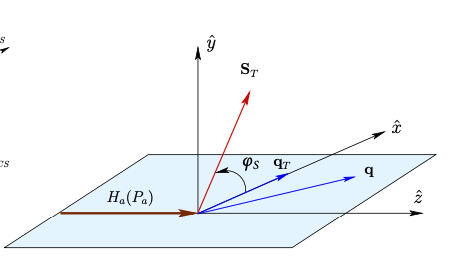
\includegraphics[width = 7.0 cm]{imgs/phi_angle.png}
    \caption{$\phi_{S}$ definition in the target rest frame.\citeme{Longo:2017snu}}
\end{figure}
\end{textblock}

\begin{textblock}{7.0}(8.0, 2.0)

\begin{align*}
\sigma(\phis) &\propto 1 + P A_{N} \sin(\phis + \phi) \\
A(\phis) &= \frac{\sigmaup - \sigmadown}{\sigmaup + \sigmadown} = A_{N} \sin{\phis}
\end{align*}

where $P$ is the target polarization, $\phis$ is the angle between $q_{T}$ \& $S_{T}$, $\phi$ is the spin alignment of the target.\\
\textcolor{nmsured}{We can extract the $A_{N}$ using $\sin{\phis}$ modulations.}

\end{textblock}

\end{frame}

\end{document}

%
% end document
%
